\documentclass[conference]{IEEEtran}
\IEEEoverridecommandlockouts
% The preceding line is only needed to identify funding in the first footnote. If that is unneeded, please comment it out.
\usepackage{cite}
\usepackage{amsmath,amssymb,amsfonts}
\usepackage{graphicx}
\usepackage{textcomp}
\usepackage{xcolor}
\usepackage{titlesec}

\usepackage{textcomp}
\usepackage{epsfig}
\usepackage{algpseudocode}
\usepackage{pgfplots}
\usepackage{tikz}
\pgfplotsset{width=10cm,compat=1.9}
 \usepgfplotslibrary{external}
\usepackage{amsmath}
\usepackage{mathtools}
\DeclarePairedDelimiter{\floor}{\lfloor}{\rfloor}
\usepackage[linesnumbered,ruled,vlined]{algorithm2e}
\def\BibTeX{{\rm B\kern-.05em{\sc i\kern-.025em b}\kern-.08em
    T\kern-.1667em\lower.7ex\hbox{E}\kern-.125emX}}

\usepackage[ruled,vlined]{algorithm2e}

\tikzexternalize 
\begin{document}

\title{ Probability of Knight to remain in the N*N chessboard\\
\text{\Large{DAA ASSIGNMENT-5 , GROUP 20}}
}
\author{\IEEEauthorblockN{Harsh Mahajan}
\IEEEauthorblockA{ \text{IIB2019001}}
\and
\IEEEauthorblockN{Pradhuman Singh Baid}
\IEEEauthorblockA{ \text{IIB2019002}}
\and
\IEEEauthorblockN{Vasu Gupta}
\IEEEauthorblockA{ \text{IIB2019003}}
}

\maketitle

\begin{abstract}
This Paper contains the algorithm to find out the probability that the Knight will remain inside the chessboard after exactly K steps, with the condition that it can't enter the chessboard again once it leaves the chessboard.\\ One approach has been taken and we will see both the time complexity and space complexity of this algorithm.
\end{abstract}

\section{Problem Statement}
Given an NxN chessboard and a Knight at position (x,y). The Knight has to
take exactly K steps, where at each step it chooses any of the 8 directions
uniformly at random. What is the probability that the Knight remains in
the chessboard after taking K steps, with the condition that it can’t enter
the board again once it leaves it? Solve using Dynamic programming.

\section{Introduction}
Dynamic Programming (DP) is an algorithmic technique for solving an optimization problem by breaking it down into simpler subproblems and utilizing the fact that the optimal solution to the overall problem depends upon the optimal solution to its subproblems. \\

\section{Algorithmic Design}

\subsection{ \textbf{Approach }}
\begin{enumerate}
\item  One thing that we can observe is that at every step the Knight has 8 choices to choose from. Suppose, the Knight has to take k steps and after taking the Kth step the knight reaches (x,y). There are 8 different positions from where the Knight can reach to (x,y) in one step, and they are: (x+1,y+2), (x+2,y+1), (x+2,y-1), (x+1,y-2), (x-1,y-2), (x-2,y-1), (x-2,y+1), (x-1,y+2). 
\item  The final probability after K steps will simply be equal to the (Σ probability of reaching each of these 8 positions after K-1 steps)/8.
\item We are dividing by 8 because each of these 8 positions has 8 choices and position (x,y) is one of the choices. 
\item For the positions that lie outside the board, we will either take their probabilities as 0 or simply neglect it.
\item Since we need to keep track of the probabilities at each position for every number of steps, we need Dynamic Programming to solve this problem. 
\item We are going to take two vectors parentBoard and childBoard. The vector parentBoard will store the probability of reaching (x,y) after (K) number of moves.
\item Base case:If the number of steps is 0, then the probability that the Knight will remain in the board is 1.
\end{enumerate}



\newline
\begin{algorithm}
    \caption{Calculating probability of Knight to remain in board after K steps}
    \KwIn{ N, K, x, y}
    \KwOut {Probability of Knight to remain inside chessboard  }
    \DontPrintSemicolon
    \SetKwFunction{FMain}{knightProbability}
    \SetKwProg{Fn}{Function}{:}{}
    \Fn{\FMain{$N,$K,$x,$y}}{
        
        \If{ K=0}{
            \STATE\Return{$1.0$};
        }
        vector $parentBoard$ , $childBoard$;
        \\ rowoffset[] = \{-2,-2,-1,-1,2,2,1,1\};
    	\\ coloffset[] = \{1,-1,2,-2,1,-1,2,-2\};
        \\
        \STATE cx,cy;
        \\
        \STATE $parentBoard[x][y] \gets 1.0;$
        \\
        \For{$i \gets 0$ \textbf{ to } $K-1$}{
            
             \For{$p \gets0$ \textbf{ to } $N-1$}{
               \For{$q \gets 0$ \textbf{ to } $N-1$}{
               		\STATE $moveProb\gets parentBoard[p][q]/8.0;$ 
               		\For{$w \gets 0$ \textbf{ to } $7$}{
                    \STATE $cx \gets p+rowoffset[w];$
                    \\
               		\STATE cy \gets q+coloffset[w];$
                    \\
                    \If{ cx\textgreater{}= 0  and cx \textless{} N and cy\textgreater{}=0 and cy \textless{} N}{
        	   \STATE childBoard[cx][cy]+\gets moveProb;$
              }
            } 
            } 
          
\\
          }
          \STATE $parentBoard \gets childBoard$
          \\ fill(childBoard.begin(),childBoard.end(),vector<double>(N,0.0));
        }
   \STATE $knightProb \gets 0.0;$
   \\
    \For{$p \gets0$ \textbf{ to } $N-1$}{
               \For{$q \gets 0$ \textbf{ to } $N-1$}{
               		\STATE knightProb+\gets parentBoard[p][q];$
                    }
                    }
                    \STATE \Return{knightProb};
    }
\end{algorithm}





% Continue.....
\newpage
\section{Complexity Analysis}

\subsection{ \textbf{Time Complexity}}\\

In this method, we are working on n \times$ n
elements and there are k layers considered.
So Time complexity would be O(n^2 \times$ k)

\subsection{ \textbf{Space Complexity}}\\
The size of parentBoard and childBoard vectors is n\times$ n and some constant variables are used.  \\
Therefore, Space complexity is O(n^2)\\

\begin{flushleft}
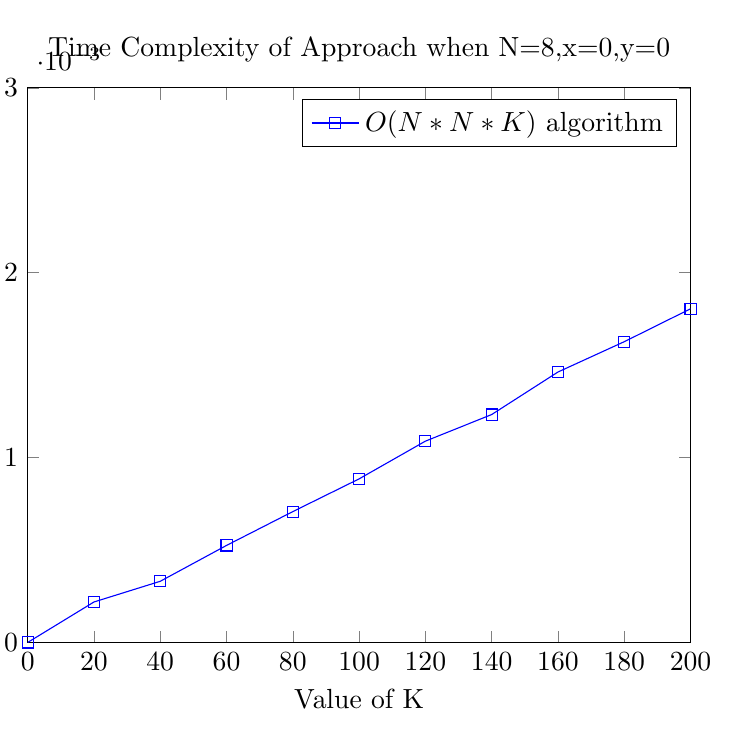
\begin{tikzpicture}[trim left=0cm]
\begin{axis}[
    title={Time Complexity of Approach when N=8,x=0,y=0 },
    xlabel={Value of K},
    ylabel={Time taken in(ms)},
    xmin=0, xmax=200,
    ymin=0, ymax=0.0030,
    xtick={0,20,40,60,80,100,120,140,160,180,200},
    ytick={0,0.0010,0.0020,0.0030}
]

\addplot[
    color=blue,
    mark=square,
    ]
    coordinates {
    (0,0)(20,0.000219)(40,0.000331)(60,0.000525)(80,0.000708)(100,0.000885)(120,0.001089)(140,0.001233)
    (160,0.001463)(180,0.001627)(200,0.001805)
    };
    \legend{$\displaystyle{O}{\left({N}*{N}*{K}\right)}$ algorithm}
   \end{axis}
   
\end{tikzpicture}
\end{flushleft}





\section{Conclusion}
This Dynamic Programming solution of Probability of Knight to remain in NxN chessboard after K steps has Time Complexity O(n^2 \times$k) and Space Complexity O(n^2).
\section{REFERENCES}\\
\textit{1) 'Dynamic Programming',Wikipedia}\\
\textit{2) 'Dynamic Programming',GeeksforGeeks}\\
\textit{3) Avinash Kumar Saw,'Probability of knight to remain in chessboard,GeeksforGeeks,2020}
\end{document}